\subsection{自律型再グループ化}
グループ内で,GLを交代し電力の平準化を図る自律型グループ化\ref{fig:group_reconstruction_independently}について述べる.全センサノードは,LoRaWAN及びBLEでの通信回数を保持している.(電力式)により,総消費電力量を見積もり可能となる.GLノードはGMノード通信時に総消費電力量を取得する.GLはGMノードの消費電力量を基に,最も消費が少ないGMノードを次のGLとして選出したのちGMへ通知する.後にデータを集約しGWへ送信する.これにより,グループ内でのセンサノードの消費電力を平準化が見込める.

\begin{figure}[]
    \begin{center}
    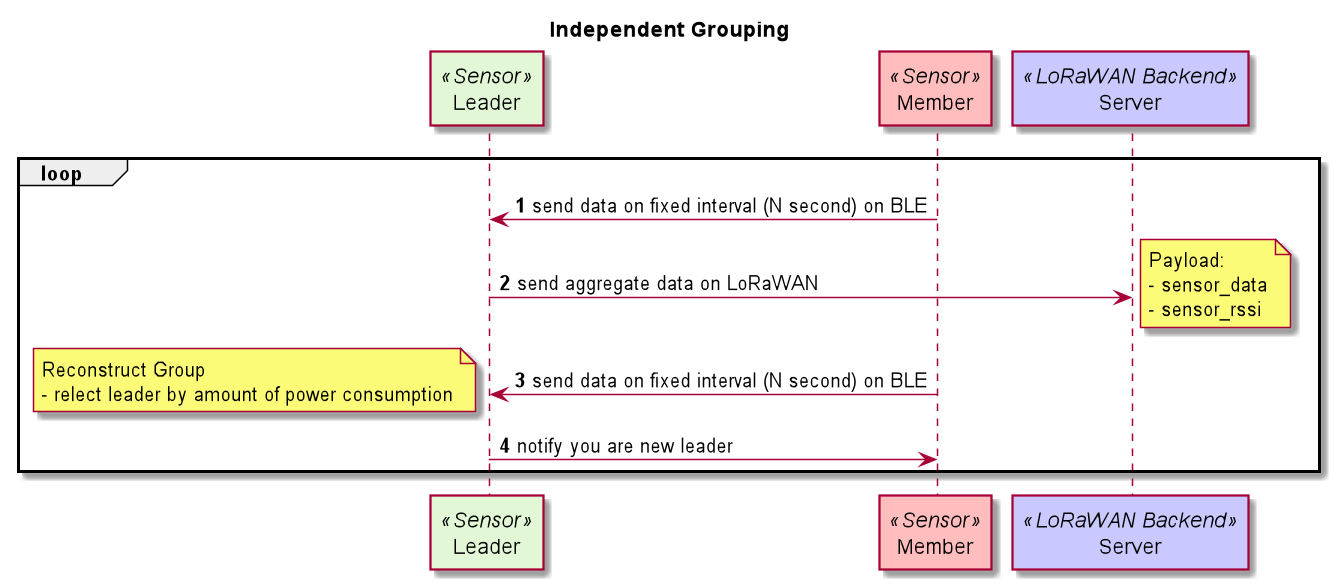
\includegraphics[width=14cm]{figures/グループ化_自律的.png}
    \caption{自律型再グループ化}
    \label{fig:group_reconstruction_independently}
    \end{center}
\end{figure}